% Options for packages loaded elsewhere
\PassOptionsToPackage{unicode}{hyperref}
\PassOptionsToPackage{hyphens}{url}
%
\documentclass[
]{article}
\usepackage{amsmath,amssymb}
\usepackage{lmodern}
\usepackage{iftex}
\ifPDFTeX
  \usepackage[T1]{fontenc}
  \usepackage[utf8]{inputenc}
  \usepackage{textcomp} % provide euro and other symbols
\else % if luatex or xetex
  \usepackage{unicode-math}
  \defaultfontfeatures{Scale=MatchLowercase}
  \defaultfontfeatures[\rmfamily]{Ligatures=TeX,Scale=1}
\fi
% Use upquote if available, for straight quotes in verbatim environments
\IfFileExists{upquote.sty}{\usepackage{upquote}}{}
\IfFileExists{microtype.sty}{% use microtype if available
  \usepackage[]{microtype}
  \UseMicrotypeSet[protrusion]{basicmath} % disable protrusion for tt fonts
}{}
\makeatletter
\@ifundefined{KOMAClassName}{% if non-KOMA class
  \IfFileExists{parskip.sty}{%
    \usepackage{parskip}
  }{% else
    \setlength{\parindent}{0pt}
    \setlength{\parskip}{6pt plus 2pt minus 1pt}}
}{% if KOMA class
  \KOMAoptions{parskip=half}}
\makeatother
\usepackage{xcolor}
\usepackage[margin=1in]{geometry}
\usepackage{graphicx}
\makeatletter
\def\maxwidth{\ifdim\Gin@nat@width>\linewidth\linewidth\else\Gin@nat@width\fi}
\def\maxheight{\ifdim\Gin@nat@height>\textheight\textheight\else\Gin@nat@height\fi}
\makeatother
% Scale images if necessary, so that they will not overflow the page
% margins by default, and it is still possible to overwrite the defaults
% using explicit options in \includegraphics[width, height, ...]{}
\setkeys{Gin}{width=\maxwidth,height=\maxheight,keepaspectratio}
% Set default figure placement to htbp
\makeatletter
\def\fps@figure{htbp}
\makeatother
\setlength{\emergencystretch}{3em} % prevent overfull lines
\providecommand{\tightlist}{%
  \setlength{\itemsep}{0pt}\setlength{\parskip}{0pt}}
\setcounter{secnumdepth}{5}
\usepackage{setspace}
\usepackage{multicol}
\usepackage{caption}
\usepackage[italian]{babel}
\usepackage{graphicx}
\usepackage{subcaption}
\ifLuaTeX
  \usepackage{selnolig}  % disable illegal ligatures
\fi
\usepackage[style=numeric,]{biblatex}
\addbibresource{bibliografia/biblioprova.bib}
\IfFileExists{bookmark.sty}{\usepackage{bookmark}}{\usepackage{hyperref}}
\IfFileExists{xurl.sty}{\usepackage{xurl}}{} % add URL line breaks if available
\urlstyle{same} % disable monospaced font for URLs
\hypersetup{
  hidelinks,
  pdfcreator={LaTeX via pandoc}}

\author{}
\date{\vspace{-2.5em}}

\begin{document}

\pagenumbering{gobble}

%\begin{titlepage}
	\begin{center}
		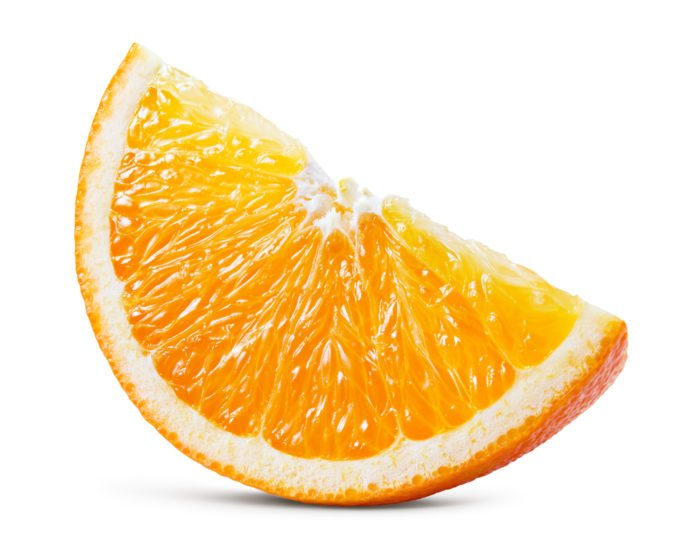
\includegraphics[width=0.25\linewidth]{img/Logo.jpg}
	\end{center}
	
	\begin{center}
		\begin{Large}
			\textbf{University of Padova}
			
			Department of Developmental Psychology and Socialisation (DPSS)
		\end{Large}
		
	\end{center}
	
	\vspace{3mm}
	\begin{center}
		\begin{large}
			Ph.D. Course in Psychological Sciences (XXXV Cycle)
		\end{large}
		
		\begin{huge}
			\bfseries
			Ideology and Moral Framing Effect on the Reaction to Different Social Threats
		\end{huge}
		
		
	\end{center}
	
	\vspace{2cm}
	\begin{multicols}{2}
		\begin{flushleft}
%			\begin{large}
				\textbf{Advisor:} Prof Luigi Castelli
				
				\textbf{Co-Advisor:} Prof Luciana Carraro
	%		\end{large}
			
		\end{flushleft}
		\columnbreak
		\begin{flushright}
			\vspace{1.5cm}
			
				\textbf{Ph.D. Candidate:} Alessia Valmori 
			
		\end{flushright}
		
	\end{multicols}

\vspace{2cm}
	
	\begin{center}
		Academic Year: 2022/2023
	\end{center}
	
	

\hypersetup{linkcolor = black}
\newpage
\renewcommand{\contentsname}{Indice}
\pagenumbering{roman}
\tableofcontents
\addcontentsline{toc}{section}{\contentsname}

\newpage

% list of figures have to be added manually to table of contents
\listoffigures % Per toogliere la lista delle figura, aggiungere % all'inizio della riga

\newpage
\listoftables % Per togliere la lista delle tabelle, aggiungere % all'inizio della riga

\doublespacing

\newpage
\pagenumbering{arabic}
\hypersetup{linkcolor = blue}

\hypertarget{introduzione}{%
\section{Introduzione}\label{introduzione}}

Ci sono varie arancette appese alla Figura \ref{fig:arancio}. Poi ci
sono arancette raccolte alla Figura \ref{sub:arance} e il plot di tutte
queste arancette alla Figura \ref{sub:grafico}.

\begin{figure}
\centering
\caption{Arancette su albero}
\label{fig:arancio} % etichetta che permette di richiamare la figura

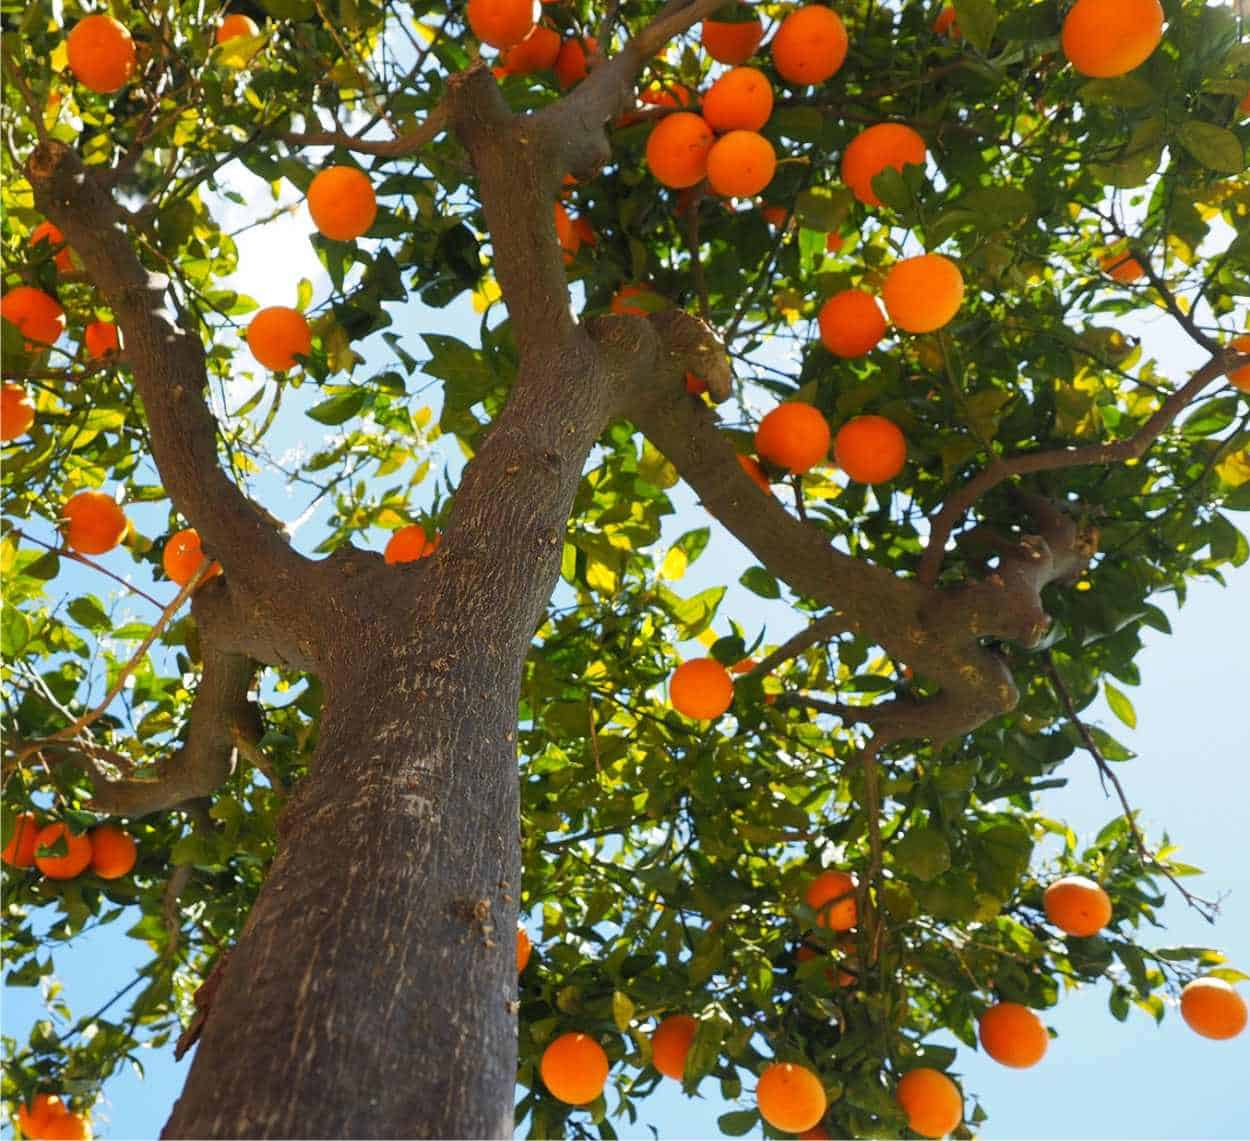
\includegraphics[width=0.5\linewidth]{img/Arancio} 
\end{figure}

\begin{figure}
\centering 
\begin{subfigure}{0.3\textwidth}

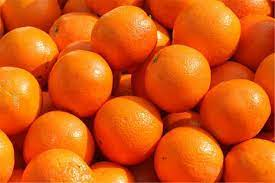
\includegraphics[width=0.8\linewidth]{img/Arance} 
\caption{Arancette raccolte} 
\label{sub:arance}
\end{subfigure} 
\begin{subfigure}{0.3\textwidth} 

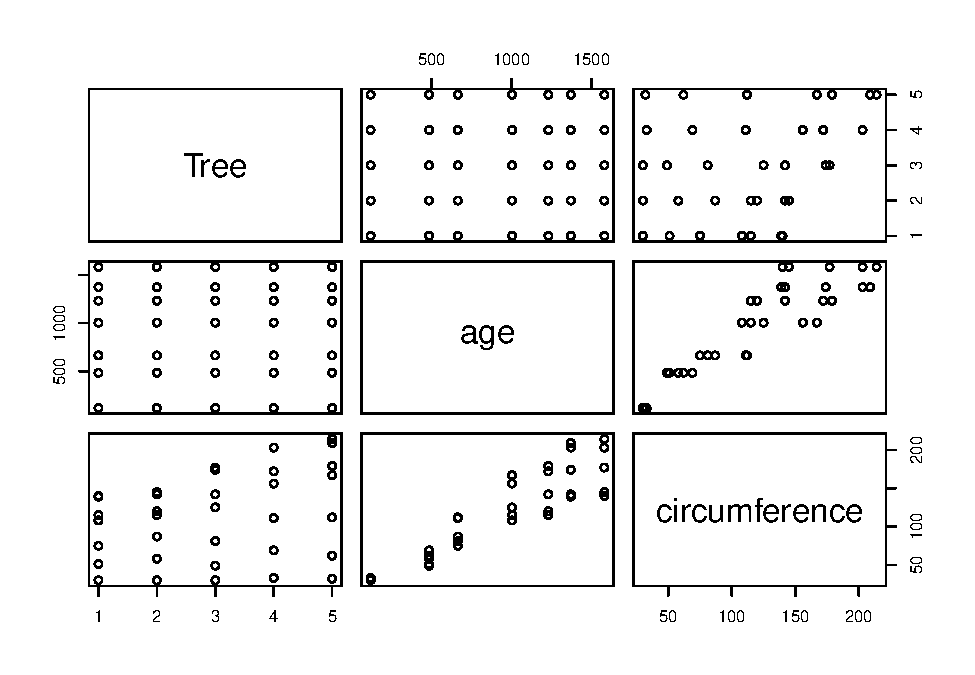
\includegraphics[width=0.8\linewidth]{Arancette_latex_files/figure-latex/unnamed-chunk-3-1} 
\caption{Grafico arancette} 
\label{sub:grafico} 
\end{subfigure} 
\end{figure}

\newpage

\hypertarget{metodo}{%
\section{Metodo}\label{metodo}}

In Equazione \ref{eq:stand} è riportata la formula della
standardizzazione.

\begin{equation}
\label{eq:stand}
z=\frac{x_i-\bar{X}}{sd}
\end{equation}

\newpage

\hypertarget{risultati}{%
\section{Risultati}\label{risultati}}

I risultati sono riportati in Tabella \ref{tab:tabella}

\begin{table}[ht]
\centering
\caption{Tabella delle arancette} 
\label{tab:tabella}
\begin{tabular}{rlrr}
  \hline
 & Tree & age & circumference \\ 
  \hline
1 & 1 & 118.00 & 30.00 \\ 
  2 & 1 & 484.00 & 58.00 \\ 
  3 & 1 & 664.00 & 87.00 \\ 
  4 & 1 & 1004.00 & 115.00 \\ 
  5 & 1 & 1231.00 & 120.00 \\ 
  6 & 1 & 1372.00 & 142.00 \\ 
  7 & 1 & 1582.00 & 145.00 \\ 
   \hline
\end{tabular}
\end{table}
\newpage

\printbibliography

\end{document}
